\documentclass[]{article}
\usepackage{graphicx}
\usepackage{amsmath}
%opening
\title{CSC420 Assignment 3}
\author{Alex (Kao-Tsun) Chang}


\begin{document}

\maketitle


\section{}

From wikipedia: Size of the 5 dollar canadian bill is height: 69.85 mm and width: 152.4 mm
\\ \\ We round to 700 x 1524 pixels, 1 per 1/10 of a mm. 
\\ \\ From the output of q1, we can see that the bill is roughly $45 \% $ of the shoe in length. We can also so that it is roughly $80 \% $ of the shoe in width. 
Measuring the pixels, we can see that the estimated shoe size is roughly\\
26cm in length
10.5cm in width

\begin{figure}[h!]
\centering
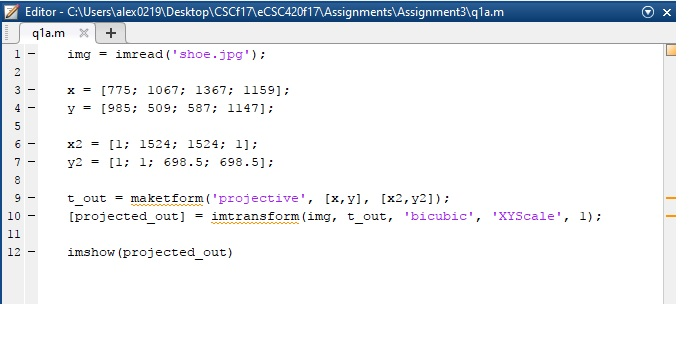
\includegraphics[width=1.35\textwidth]{img/q1code.jpg}
\caption{Projection matlab code for q1}
\end{figure}


\begin{figure}[h!]
\centering
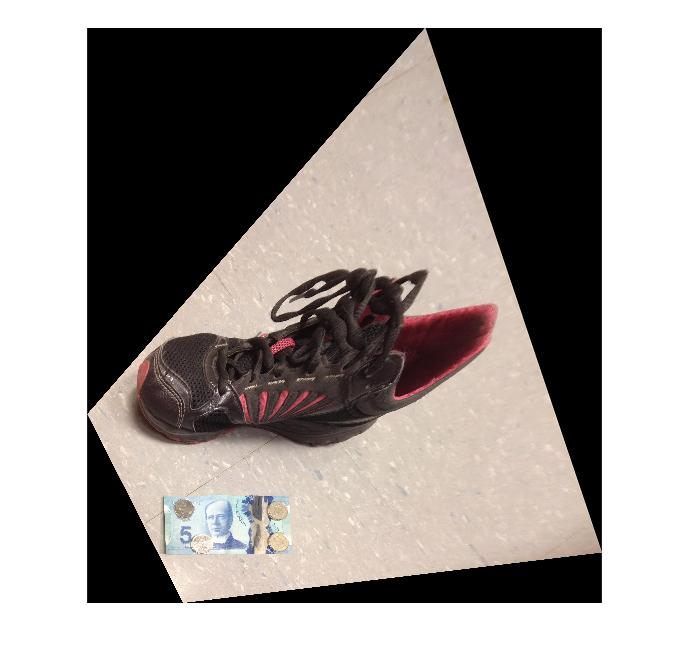
\includegraphics[width=1.15\textwidth]{img/q1.jpg}
\caption{Output}
\end{figure}

\section{}
\begin{figure}[h!]
\centering
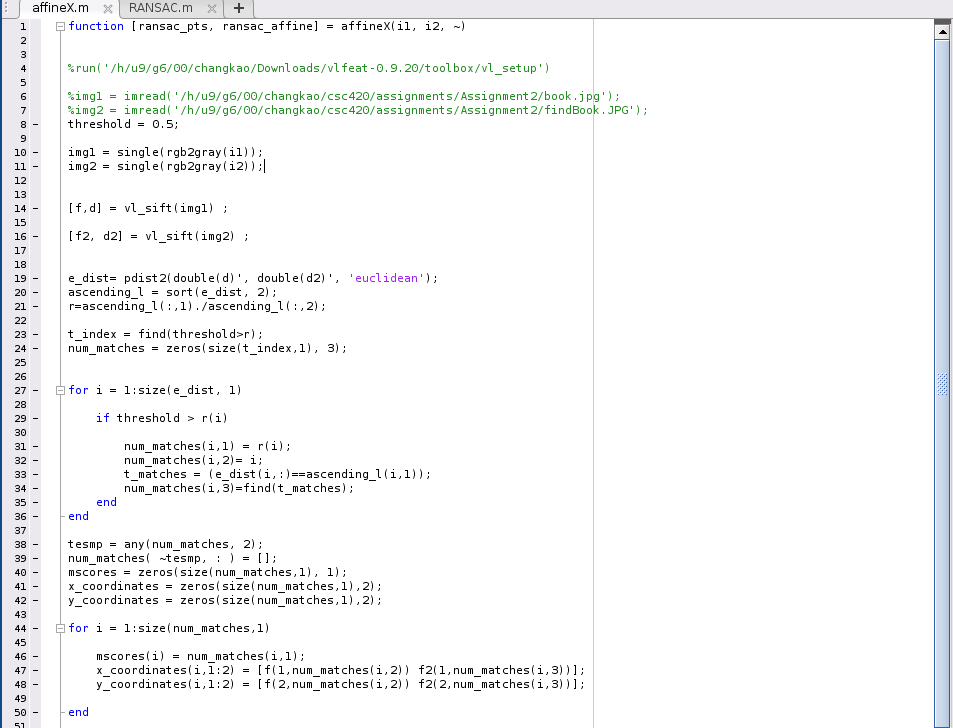
\includegraphics[width=1.35\textwidth]{img/affine1.png}
\caption{main function - RANSAC code matlab part 1}
\end{figure}

\begin{figure}[h!]
\centering
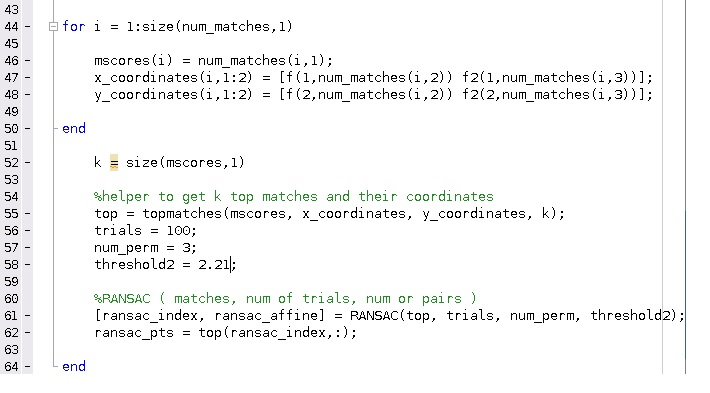
\includegraphics[width=1.35\textwidth]{img/affine2.jpg}
\caption{main function - RANSAC code matlab part 2}
\end{figure}

\begin{figure}[h!]
\centering
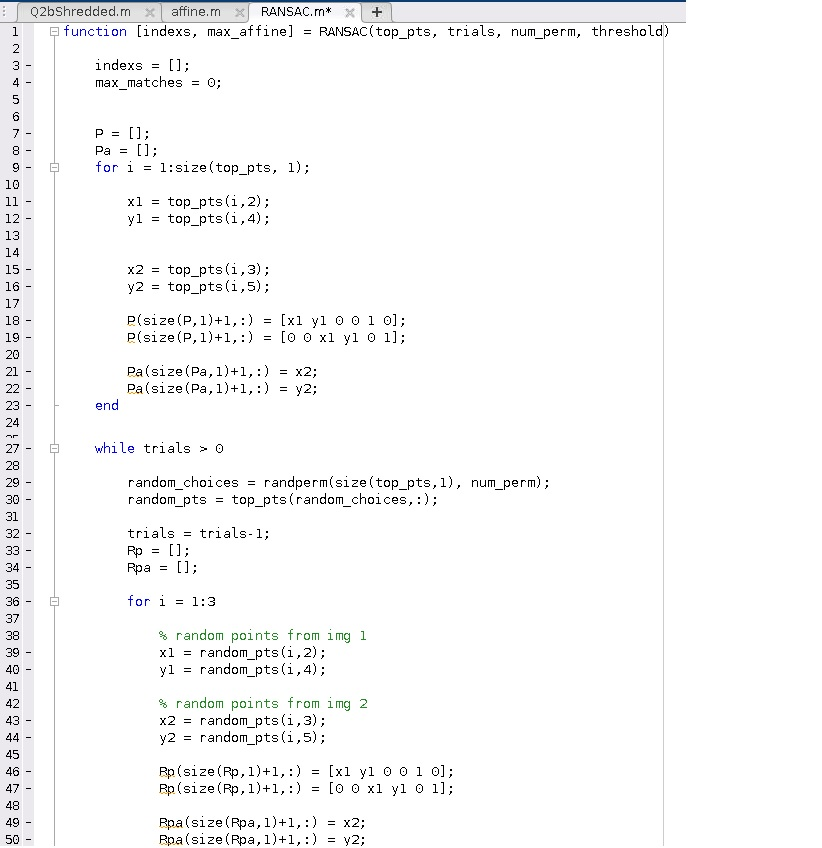
\includegraphics[width=1.35\textwidth]{img/ransac1.jpg}
\caption{RANSAC code matlab part 1}
\end{figure}

\begin{figure}[h!]
\centering
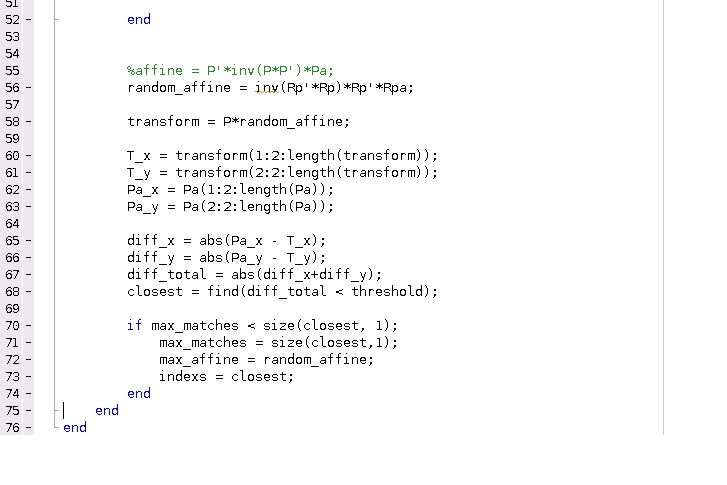
\includegraphics[width=1.35\textwidth]{img/ransac2.jpg}
\caption{RANSAC code matlab part 2}
\end{figure}

(a + b)
\begin{figure}[h!]
\centering
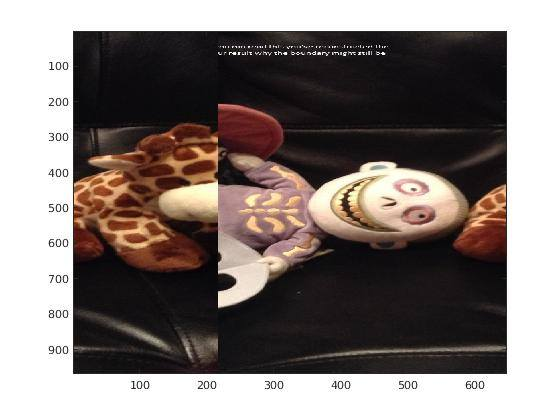
\includegraphics[width=1.35\textwidth]{img/shredded.jpg}
\caption{Output - 100 trials, 0.68 threshold}
\end{figure}

\end{document}
